% (C) Marc Lijour, 2016-2017 
% Licensed under a Creative Commons License BY-SA
% https://creativecommons.org/licenses/by-sa/2.5/ca/
% Presentation for the Small Business Digitization Initiative (SBDI) training program
% see http://www.ictc-ctic.ca/small-business-digitization-initiative/ 
% authored by Marc Lijour, April 2017
% for the session running from January 2017 to September 2017
% 
% Variables
% TODO set the variables
% ---------------------- USER-DEFINED --------------------------------
\newcommand{\SFLtitle}{Digitization~Theory~1}
\newcommand{\SFLlongtitle}{Introduction to Odoo: the course ERP}
\newcommand{\SFLsubtitle}{Small Business Digitization Initiative (SBDI)}
\newcommand{\SFLauthor}{Marc~Lijour}
\newcommand{\SFLdate}{April~19, 2017}
\newcommand{\SFLsubject}{Digitization Theory}
% --------------------------------------------------------------------
% Template
% (C) Savoir-faire Linux, 2016 (this document and associated logos and art)
% This document is licensed under a Creative Commons License BY-SA (feel free to use the code, but all rights are reserved for logos and art)
% https://creativecommons.org/licenses/by-sa/2.5/ca/
% Savoir-faire Linux presentation template for LaTeX
% authored by Marc Lijour, December 2016
% This template comes with a first page on a blue background
% Possible improvement in future iterations
% - Test and fix as needed to work on xetex (to use Ubuntu fonts)
% === USAGE===
% Create a file for your LaTeX content (slides, etc), in which you must do the following:
% TODO 1 - set variables defined below
% TODO 2 - include this code by calling: % (C) Savoir-faire Linux, 2016 (this document and associated logos and art)
% This document is licensed under a Creative Commons License BY-SA (feel free to use the code, but all rights are reserved for logos and art)
% https://creativecommons.org/licenses/by-sa/2.5/ca/
% Savoir-faire Linux presentation template for LaTeX
% authored by Marc Lijour, December 2016
% This template comes with a first page on a blue background
% Possible improvement in future iterations
% - Test and fix as needed to work on xetex (to use Ubuntu fonts)
% === USAGE===
% Create a file for your LaTeX content (slides, etc), in which you must do the following:
% TODO 1 - set variables defined below
% TODO 2 - include this code by calling: % (C) Savoir-faire Linux, 2016 (this document and associated logos and art)
% This document is licensed under a Creative Commons License BY-SA (feel free to use the code, but all rights are reserved for logos and art)
% https://creativecommons.org/licenses/by-sa/2.5/ca/
% Savoir-faire Linux presentation template for LaTeX
% authored by Marc Lijour, December 2016
% This template comes with a first page on a blue background
% Possible improvement in future iterations
% - Test and fix as needed to work on xetex (to use Ubuntu fonts)
% === USAGE===
% Create a file for your LaTeX content (slides, etc), in which you must do the following:
% TODO 1 - set variables defined below
% TODO 2 - include this code by calling: \input{sfl-presentation-template-blue-EN}
% TODO 3 - Start the document as usual and you're in business; just use \begin{document} and don't forget to conclude with \end{document}
% TODO 4 - Use the custom method \SFLcoverpage instead of \titlepage to create your cover page
% Voilà!
%
\documentclass{beamer}
\usepackage{etoolbox}
% Variables
% ---------------------- USER-DEFINED --------------------------------
\ifdef{\SFLtitle}{}{\newcommand{\SFLtitle}{\color{red}Title TBD}}
\ifdef{\SFLlongtitle}{}{\newcommand{\SFLlongtitle}{\color{red}Long title TBD}}
\ifdef{\SFLsubtitle}{}{\newcommand{\SFLsubtitle}{\color{red}Subtitle TBD}}
\ifdef{\SFLauthor}{}{\newcommand{\SFLauthor}{\color{red}Author TBD}}
\ifdef{\SFLdate}{}{\newcommand{\SFLdate}{\color{red}Date TBD}}
\ifdef{\SFLsubject}{}{\newcommand{\SFLsubject}{\color{red}Subject TBD}}
% --------------------------------------------------------------------
\usetheme{Boadilla}
% Set color close to Savoir-faire Linux standard
\definecolor{beamer@blendedblue}{RGB}{86,176,201}
% Cover Page
\title[\SFLtitle] {\SFLlongtitle}
\subtitle{\SFLsubtitle}
\author{\SFLauthor}
\date{\SFLdate}
\subject{\SFLsubject}
\usepackage{tikz}
% -- possible approach through modif of the template (abandonned for now)
%\addtobeamertemplate{title page}{
%    \tikz[remember picture,overlay]
%        \node at ([xshift=0cm,yshift=0cm]current page.center) 
%		 {
\includegraphics[width=\paperwidth, height=\paperheight]{./images/sfl-background-blue}};
%}{}
%\setbeamercolor{title page}{fg=white}
%\setbeamercolor{titlelike}{fg=white}
%\setbeamertemplate{navigation symbols}{}
% Try Xetex to use system fonts (pdflatex makes it hard to import a font)
%\usepackage{fontspec}
%\setsansfont{Ubuntu}
%\setmonofont{Ubuntu Mono}
%
%\usepackage[absolute,overlay]{textpos}
%\setlength{\TPHorizModule}{\paperwidth}
%\setlength{\TPVertModule}{\paperheight}
% -- create a custom (command) title page -which has the benefit of not affecting the settings for the rest of the presentation
\newcommand{\SFLcoverpage}{\frame[plain]{
	\tikz[remember picture,overlay] {
        	\node(bkgd) at ([xshift=0cm,yshift=0cm]current page.center) 
			{
\includegraphics[width=\paperwidth, height=\paperheight]{../templates/images/sfl-background-blue}};
        	\node(logo) at ([xshift=0cm,yshift=2.5cm]current page.center) 
		 	{
\includegraphics[scale=.20]{../templates/images/logo-sfl-blanc-rgb-72dpi}};
	}
	\tikz[remember picture,overlay] {
        	\node(title) at ([xshift=0cm,yshift=1cm]current page.center) 
			{\Large\color{white}\textbf{{\SFLlongtitle}}};
        	\node(subtitle) at ([xshift=0cm,yshift=.2cm]current page.center) 
			{\small\color{white}\emph{\SFLsubtitle}};
        	\node(author) at ([xshift=0cm,yshift=-2cm]current page.center) 
			{\small\color{white}By~\SFLauthor};
        	\node(date) at ([xshift=0cm,yshift=-2.5cm]current page.center) 
			{\tiny\color{white}\SFLdate};
        	\node(footnote) at ([xshift=0cm,yshift=-4cm]current page.center) 
			{\TINY\color{white}\emph{The registered trademark Linux$^\circledR$ is used pursuant to a sublicense from LMI, the exclusive licensee of Linus Torvalds, owner of the mark on a world-wide basis.}};
    	}
}}
%
% This sets a Savoir-faire Linux logo at the bottom right corner of each page
\logo{
\includegraphics[scale=.1]{../templates/images/logo-sfl-250.png}}
\AtBeginSection[]
{
  \begin{frame}
    \frametitle{Table of Contents}
    \tableofcontents[currentsection]
  \end{frame}
}
%\usepackage[format=plain,justification=raggedright,singlelinecheck=false]{caption}
\usepackage[format=plain,justification=justified,singlelinecheck=false]{caption}
\usepackage[utf8]{inputenc}
\usepackage{dirtytalk}
\usepackage{wrapfig}
\usepackage{hyperref}
\usepackage{verbatim}
\usepackage{mathabx}
%\usepackage{MnSymbol}


% TODO 3 - Start the document as usual and you're in business; just use \begin{document} and don't forget to conclude with \end{document}
% TODO 4 - Use the custom method \SFLcoverpage instead of \titlepage to create your cover page
% Voilà!
%
\documentclass{beamer}
\usepackage{etoolbox}
% Variables
% ---------------------- USER-DEFINED --------------------------------
\ifdef{\SFLtitle}{}{\newcommand{\SFLtitle}{\color{red}Title TBD}}
\ifdef{\SFLlongtitle}{}{\newcommand{\SFLlongtitle}{\color{red}Long title TBD}}
\ifdef{\SFLsubtitle}{}{\newcommand{\SFLsubtitle}{\color{red}Subtitle TBD}}
\ifdef{\SFLauthor}{}{\newcommand{\SFLauthor}{\color{red}Author TBD}}
\ifdef{\SFLdate}{}{\newcommand{\SFLdate}{\color{red}Date TBD}}
\ifdef{\SFLsubject}{}{\newcommand{\SFLsubject}{\color{red}Subject TBD}}
% --------------------------------------------------------------------
\usetheme{Boadilla}
% Set color close to Savoir-faire Linux standard
\definecolor{beamer@blendedblue}{RGB}{86,176,201}
% Cover Page
\title[\SFLtitle] {\SFLlongtitle}
\subtitle{\SFLsubtitle}
\author{\SFLauthor}
\date{\SFLdate}
\subject{\SFLsubject}
\usepackage{tikz}
% -- possible approach through modif of the template (abandonned for now)
%\addtobeamertemplate{title page}{
%    \tikz[remember picture,overlay]
%        \node at ([xshift=0cm,yshift=0cm]current page.center) 
%		 {
\includegraphics[width=\paperwidth, height=\paperheight]{./images/sfl-background-blue}};
%}{}
%\setbeamercolor{title page}{fg=white}
%\setbeamercolor{titlelike}{fg=white}
%\setbeamertemplate{navigation symbols}{}
% Try Xetex to use system fonts (pdflatex makes it hard to import a font)
%\usepackage{fontspec}
%\setsansfont{Ubuntu}
%\setmonofont{Ubuntu Mono}
%
%\usepackage[absolute,overlay]{textpos}
%\setlength{\TPHorizModule}{\paperwidth}
%\setlength{\TPVertModule}{\paperheight}
% -- create a custom (command) title page -which has the benefit of not affecting the settings for the rest of the presentation
\newcommand{\SFLcoverpage}{\frame[plain]{
	\tikz[remember picture,overlay] {
        	\node(bkgd) at ([xshift=0cm,yshift=0cm]current page.center) 
			{
\includegraphics[width=\paperwidth, height=\paperheight]{../templates/images/sfl-background-blue}};
        	\node(logo) at ([xshift=0cm,yshift=2.5cm]current page.center) 
		 	{
\includegraphics[scale=.20]{../templates/images/logo-sfl-blanc-rgb-72dpi}};
	}
	\tikz[remember picture,overlay] {
        	\node(title) at ([xshift=0cm,yshift=1cm]current page.center) 
			{\Large\color{white}\textbf{{\SFLlongtitle}}};
        	\node(subtitle) at ([xshift=0cm,yshift=.2cm]current page.center) 
			{\small\color{white}\emph{\SFLsubtitle}};
        	\node(author) at ([xshift=0cm,yshift=-2cm]current page.center) 
			{\small\color{white}By~\SFLauthor};
        	\node(date) at ([xshift=0cm,yshift=-2.5cm]current page.center) 
			{\tiny\color{white}\SFLdate};
        	\node(footnote) at ([xshift=0cm,yshift=-4cm]current page.center) 
			{\TINY\color{white}\emph{The registered trademark Linux$^\circledR$ is used pursuant to a sublicense from LMI, the exclusive licensee of Linus Torvalds, owner of the mark on a world-wide basis.}};
    	}
}}
%
% This sets a Savoir-faire Linux logo at the bottom right corner of each page
\logo{
\includegraphics[scale=.1]{../templates/images/logo-sfl-250.png}}
\AtBeginSection[]
{
  \begin{frame}
    \frametitle{Table of Contents}
    \tableofcontents[currentsection]
  \end{frame}
}
%\usepackage[format=plain,justification=raggedright,singlelinecheck=false]{caption}
\usepackage[format=plain,justification=justified,singlelinecheck=false]{caption}
\usepackage[utf8]{inputenc}
\usepackage{dirtytalk}
\usepackage{wrapfig}
\usepackage{hyperref}
\usepackage{verbatim}
\usepackage{mathabx}
%\usepackage{MnSymbol}


% TODO 3 - Start the document as usual and you're in business; just use \begin{document} and don't forget to conclude with \end{document}
% TODO 4 - Use the custom method \SFLcoverpage instead of \titlepage to create your cover page
% Voilà!
%
\documentclass{beamer}
\usepackage{etoolbox}
% Variables
% ---------------------- USER-DEFINED --------------------------------
\ifdef{\SFLtitle}{}{\newcommand{\SFLtitle}{\color{red}Title TBD}}
\ifdef{\SFLlongtitle}{}{\newcommand{\SFLlongtitle}{\color{red}Long title TBD}}
\ifdef{\SFLsubtitle}{}{\newcommand{\SFLsubtitle}{\color{red}Subtitle TBD}}
\ifdef{\SFLauthor}{}{\newcommand{\SFLauthor}{\color{red}Author TBD}}
\ifdef{\SFLdate}{}{\newcommand{\SFLdate}{\color{red}Date TBD}}
\ifdef{\SFLsubject}{}{\newcommand{\SFLsubject}{\color{red}Subject TBD}}
% --------------------------------------------------------------------
\usetheme{Boadilla}
% Set color close to Savoir-faire Linux standard
\definecolor{beamer@blendedblue}{RGB}{86,176,201}
% Cover Page
\title[\SFLtitle] {\SFLlongtitle}
\subtitle{\SFLsubtitle}
\author{\SFLauthor}
\date{\SFLdate}
\subject{\SFLsubject}
\usepackage{tikz}
% -- possible approach through modif of the template (abandonned for now)
%\addtobeamertemplate{title page}{
%    \tikz[remember picture,overlay]
%        \node at ([xshift=0cm,yshift=0cm]current page.center) 
%		 {
\includegraphics[width=\paperwidth, height=\paperheight]{./images/sfl-background-blue}};
%}{}
%\setbeamercolor{title page}{fg=white}
%\setbeamercolor{titlelike}{fg=white}
%\setbeamertemplate{navigation symbols}{}
% Try Xetex to use system fonts (pdflatex makes it hard to import a font)
%\usepackage{fontspec}
%\setsansfont{Ubuntu}
%\setmonofont{Ubuntu Mono}
%
%\usepackage[absolute,overlay]{textpos}
%\setlength{\TPHorizModule}{\paperwidth}
%\setlength{\TPVertModule}{\paperheight}
% -- create a custom (command) title page -which has the benefit of not affecting the settings for the rest of the presentation
\newcommand{\SFLcoverpage}{\frame[plain]{
	\tikz[remember picture,overlay] {
        	\node(bkgd) at ([xshift=0cm,yshift=0cm]current page.center) 
			{
\includegraphics[width=\paperwidth, height=\paperheight]{../templates/images/sfl-background-blue}};
        	\node(logo) at ([xshift=0cm,yshift=2.5cm]current page.center) 
		 	{
\includegraphics[scale=.20]{../templates/images/logo-sfl-blanc-rgb-72dpi}};
        	\node(CC-BY-SA) at ([xshift=5cm,yshift=-3.5cm]current page.center) 
			{\href{https://creativecommons.org/licenses/by-sa/2.5/ca/}{
\includegraphics[scale=.4]{../templates/images/CC-BY-SA-403x141}}};
	}
	\tikz[remember picture,overlay] {
        	\node(title) at ([xshift=0cm,yshift=1cm]current page.center) 
			{\Large\color{white}\textbf{{\SFLlongtitle}}};
        	\node(subtitle) at ([xshift=0cm,yshift=.2cm]current page.center) 
			{\small\color{white}\emph{\SFLsubtitle}};
        	\node(author) at ([xshift=0cm,yshift=-2cm]current page.center) 
			{\small\color{white}By~\SFLauthor};
        	\node(date) at ([xshift=0cm,yshift=-2.5cm]current page.center) 
			{\tiny\color{white}\SFLdate};
        	\node(footnote) at ([xshift=0cm,yshift=-4cm]current page.center) 
			{\TINY\color{white}\emph{The registered trademark Linux$^\circledR$ is used pursuant to a sublicense from LMI, the exclusive licensee of Linus Torvalds, owner of the mark on a world-wide basis.}};
    	}
}}
%
% This sets a Savoir-faire Linux logo at the bottom right corner of each page
\logo{
	
\includegraphics[scale=.1]{../templates/images/logo-sfl-250.png}
}
\AtBeginSection[]
{
  \begin{frame}
    \frametitle{Table of Contents}
    \tableofcontents[currentsection]
  \end{frame}
}
%\usepackage[format=plain,justification=raggedright,singlelinecheck=false]{caption}
\usepackage[format=plain,justification=justified,singlelinecheck=false]{caption}
\usepackage[utf8]{inputenc}
\usepackage{dirtytalk}
\usepackage{wrapfig}
\usepackage{hyperref}
\usepackage{verbatim}
\usepackage{mathabx}
%\usepackage{MnSymbol}


% Extra packages
\usepackage{amssymb}
\usepackage{amsmath}
\usepackage[american]{babel}
\usepackage{csquotes}
\usepackage[backend=biber,style=apa]{biblatex}
\DeclareLanguageMapping{american}{american-apa}
% Use one bib file per section
%\addbibresource{references-program-overview.bib}
\addbibresource{references-odoo-course-erp.bib}
\definecolor{links}{HTML}{2A1B81}
\hypersetup{colorlinks,linkcolor=,urlcolor=links}
% Start of the document
\begin{document}
% Cover page
% Do not use this: \frame{\titlepage}
% use this instead:
\SFLcoverpage

% (C) Marc Lijour, 2016-2017 
% Licensed under a Creative Commons License BY-SA
% https://creativecommons.org/licenses/by-sa/2.5/ca/
% Presentation for the Small Business Digitization Initiative (SBDI) training program
% see http://www.ictc-ctic.ca/small-business-digitization-initiative/ 
% authored by Marc Lijour, April 2017 
% for the session running from January 2017 to September 2017
% 
% ======================================================================================================
%                                     Odoo: What is it?
% ======================================================================================================
\section{Odoo: the course ERP}
% --------------------- Short intro --------------------------
\subsection{A Short Introduction to Odoo}
\frame{
	\frametitle{Small Business Digitization Initiative}
	\framesubtitle{Odoo -- The course ``ERP''}
	\begin{figure}
	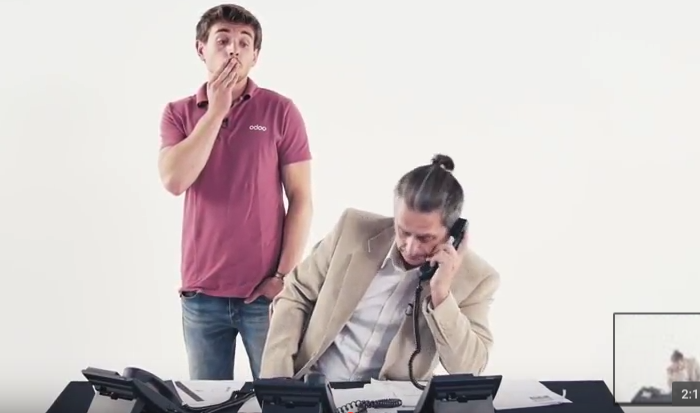
\includegraphics[width=11.5cm]{../pics/odoo-youtube-notERP}
	\caption{\tiny\url{https://www.youtube.com/watch?v=2dhyhamLm6M&list=PL1-aSABtP6AALA_4hW2TyYIioOVEGQ3yf&index=6}}
	\end{figure}
}

%\frame{
%	\frametitle{}
%	\framesubtitle{}
%}

\frame{
	\frametitle{A Short Introduction to Odoo}
	\framesubtitle{Odoo in a few words}
	\begin{figure}	
		\centering
		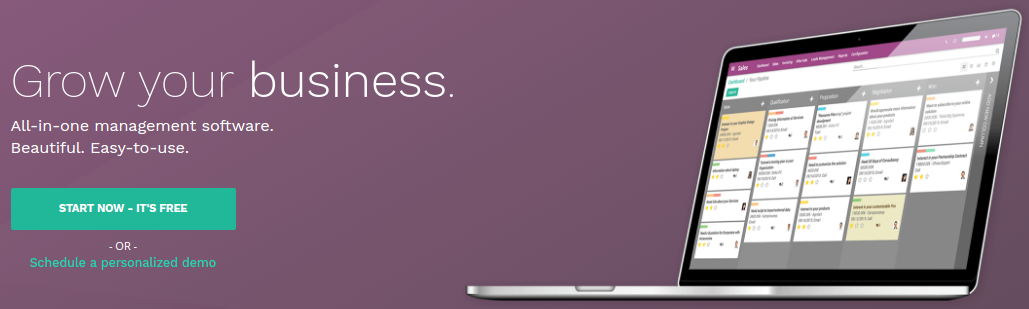
\includegraphics[width=12cm]{../pics/odoo-tagline}
		\caption{\url{https://www.odoo.com} (\cite{odoosa})}
	\end{figure}
}

\frame{
	\frametitle{A Short Introduction to Odoo}
	\framesubtitle{Value Proposition}
	\begin{figure}	
		\centering
		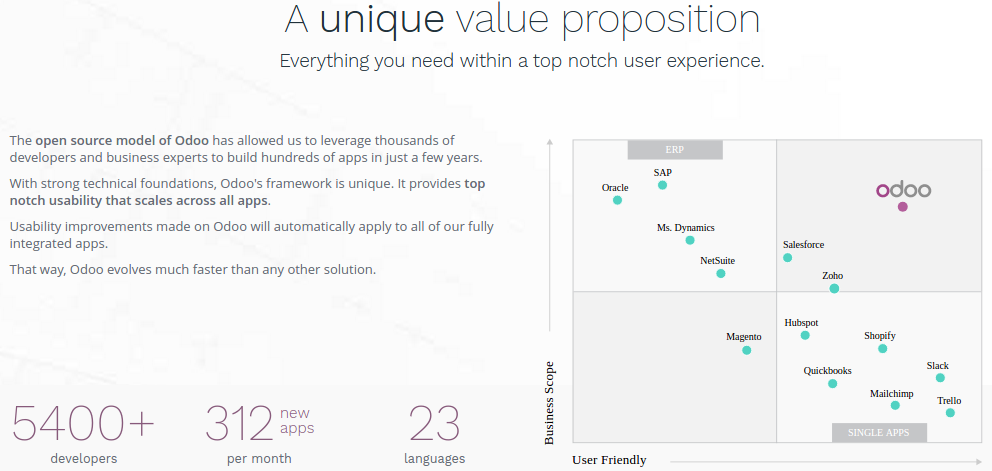
\includegraphics[width=12cm]{../pics/odoo-unique-value-prop}
	\end{figure}
}

% --------------------- Why Odoo in this course --------------------------
\subsection{Why we chose Odoo}
\frame{
	\frametitle{Why we chose Odoo}
	\framesubtitle{In a few words}
	\begin{itemize}
		\item Simple and Easy to use (and to learn)
		\pause
		\item Cheap for students (Open Source version is \$0, and Enterprise is freely available)
		\pause
		\item Cheap for employers (Enterprise: one app = \$0; other apps are affordable)
		\pause
		\item Extensible (Official apps + thousands of open source apps)
		\pause
		\item Beautiful
		\pause
		\item Odoo Community in Toronto and Montreal
	\end{itemize}
}

\frame{
	\frametitle{Why we chose Odoo}
	\framesubtitle{Odoo Communication Association (OCA)}
	\begin{figure}	
		\centering
		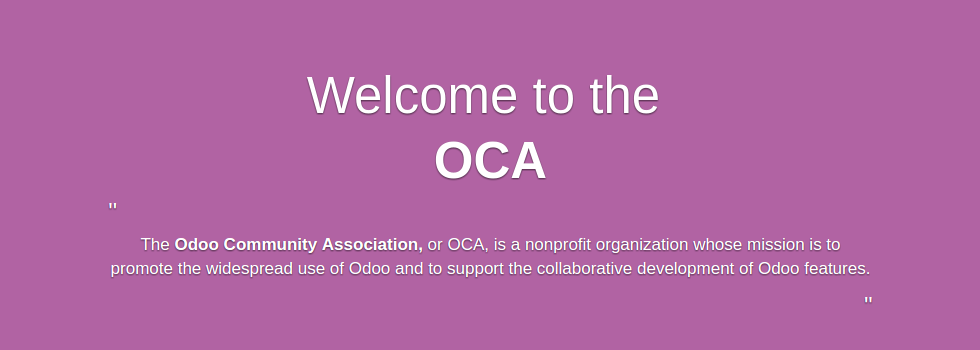
\includegraphics[width=12cm]{../pics/odoo-OCA}
		\caption{\url{https://odoo-community.org} (\cite{oca})}
	\end{figure}
}


\frame{
	\frametitle{Why we chose Odoo}
	\framesubtitle{Odoo Communication Association (OCA) Apps}
	\begin{figure}	
		\centering
		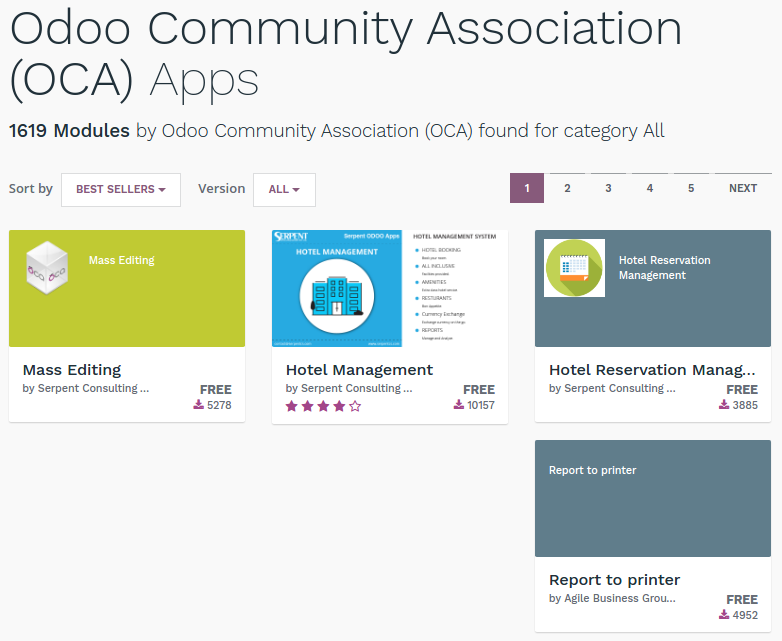
\includegraphics[height=6cm]{../pics/odoo-OCA-apps}
		\caption{See the \href{https://www.odoo.com/apps/modules?author=Odoo\%20Community\%20Association\%20(OCA)}{OCA section on Odoo.com} and \url{https://github.com/OCA} (\cite{ocagithub,ocaappsonodoo})}
	\end{figure}
}


\frame{
	\frametitle{Why we chose Odoo}
	\framesubtitle{Thousands of Open Source modules}
	\begin{figure}	
		\centering
		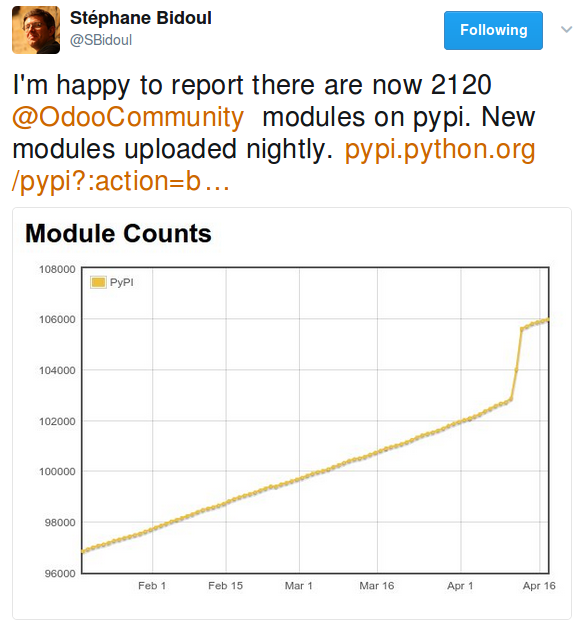
\includegraphics[height=6cm]{../pics/odoo-pypi}
	\end{figure}
}


% --------------------- Version of Odoo --------------------------
\section{Versions of Odoo}
\frame{
	\frametitle{Versions of Odoo}
	\framesubtitle{Opencore Model}
	\begin{itemize}[<+->]
		\item Odoo Community
		\item Odoo Enterprise
		\item Developer version (see Tech Labs)
	\end{itemize}
}

\frame{
	\frametitle{Versions of Odoo}
	\framesubtitle{SaaS vs. On-premise}
	\begin{itemize}[<+->]
		\item Odoo SaaS (starts with one free apps)
		\item Odoo can be installed on Enterprise Servers
	\end{itemize}
}


% --------------------- Why Odoo in this course --------------------------

% ======================================================================================================
%                                     Additional Odoo Training
% ======================================================================================================
\section{Additional Odoo Training}
\frame{
	\frametitle{Odoo Training}
	\framesubtitle{Courses on Udemy}
	\begin{figure}	
		\centering
		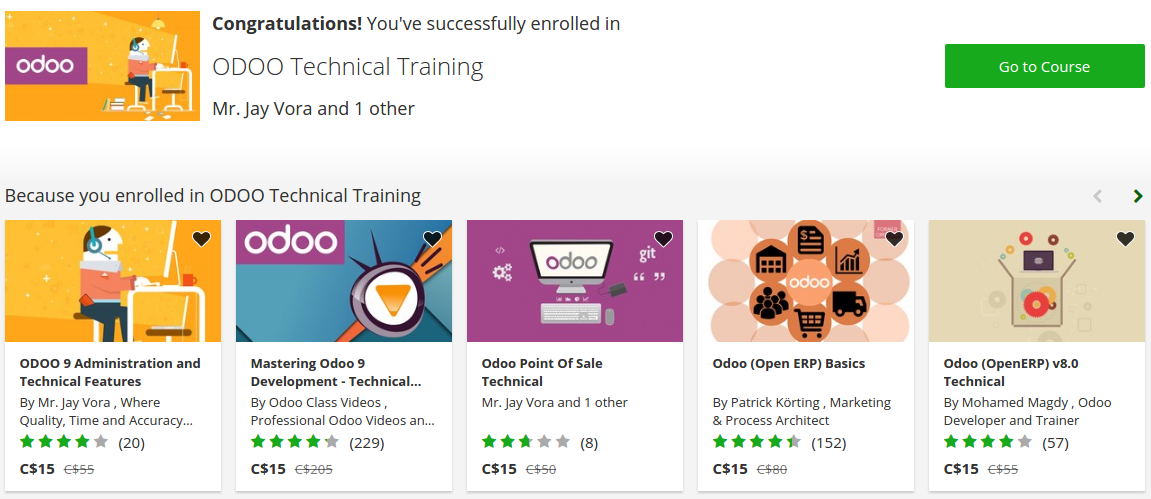
\includegraphics[width=12cm]{../pics/udemy-sample-odoo-courses}
		\caption{\tiny \url{https://www.udemy.com/odoo-technical/}}
	\end{figure}
}

\frame{
	\frametitle{Odoo Training}
	\framesubtitle{Books on O'Reilly Safari (there is plenty)}
	\begin{figure}	
		\centering
		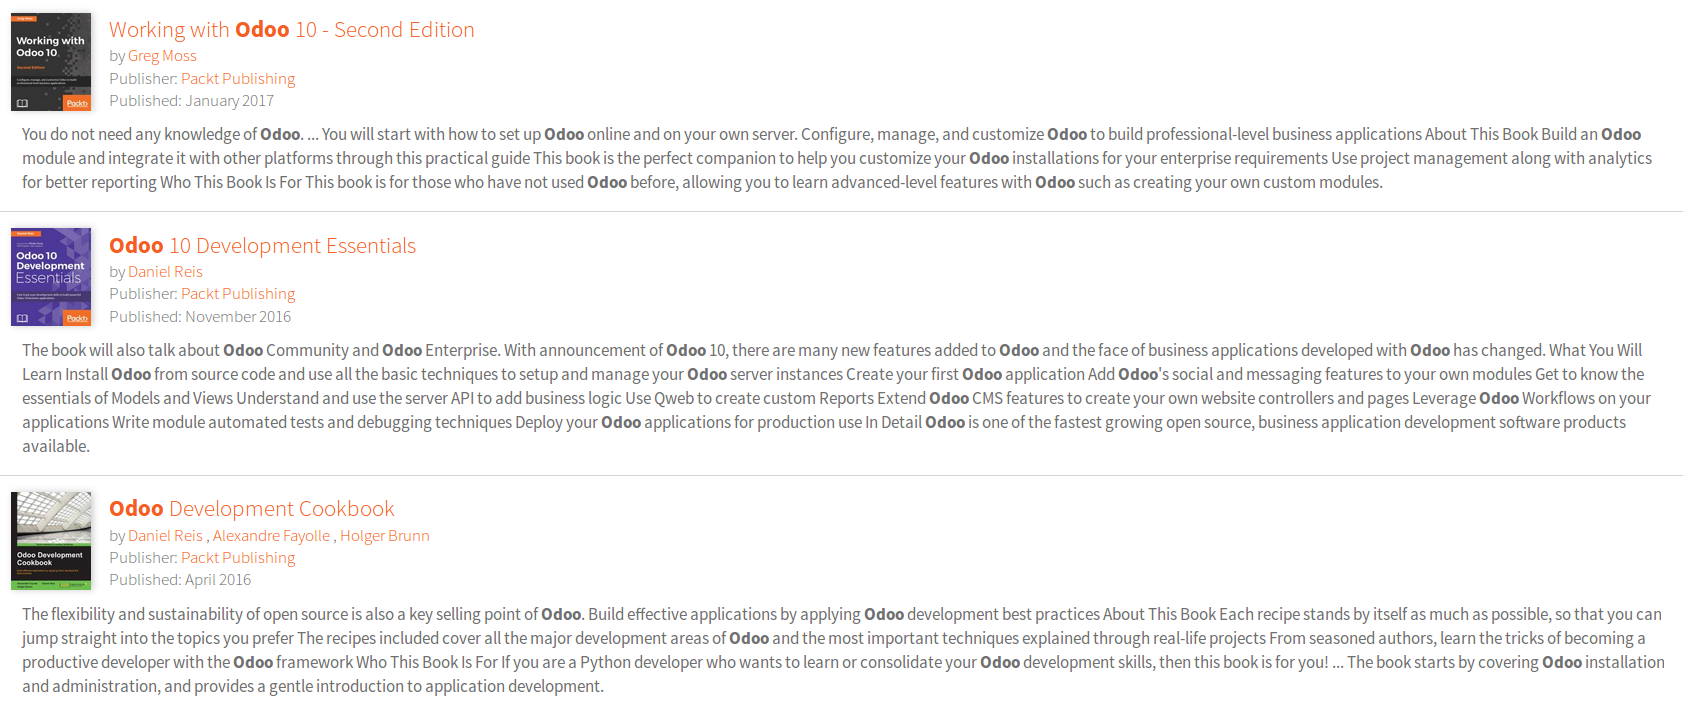
\includegraphics[width=12cm]{../pics/odoo-safari}
		\caption{\href{http://my.safaribooksonline.com/}{O'Reilly Safari} is freely accessible with a Toronto Public Library Card (\cite{oreillysafari})}
	\end{figure}
}

\frame{
	\frametitle{Odoo Training}
	\framesubtitle{from Odoo S.A.}
	\begin{figure}
		\centering
		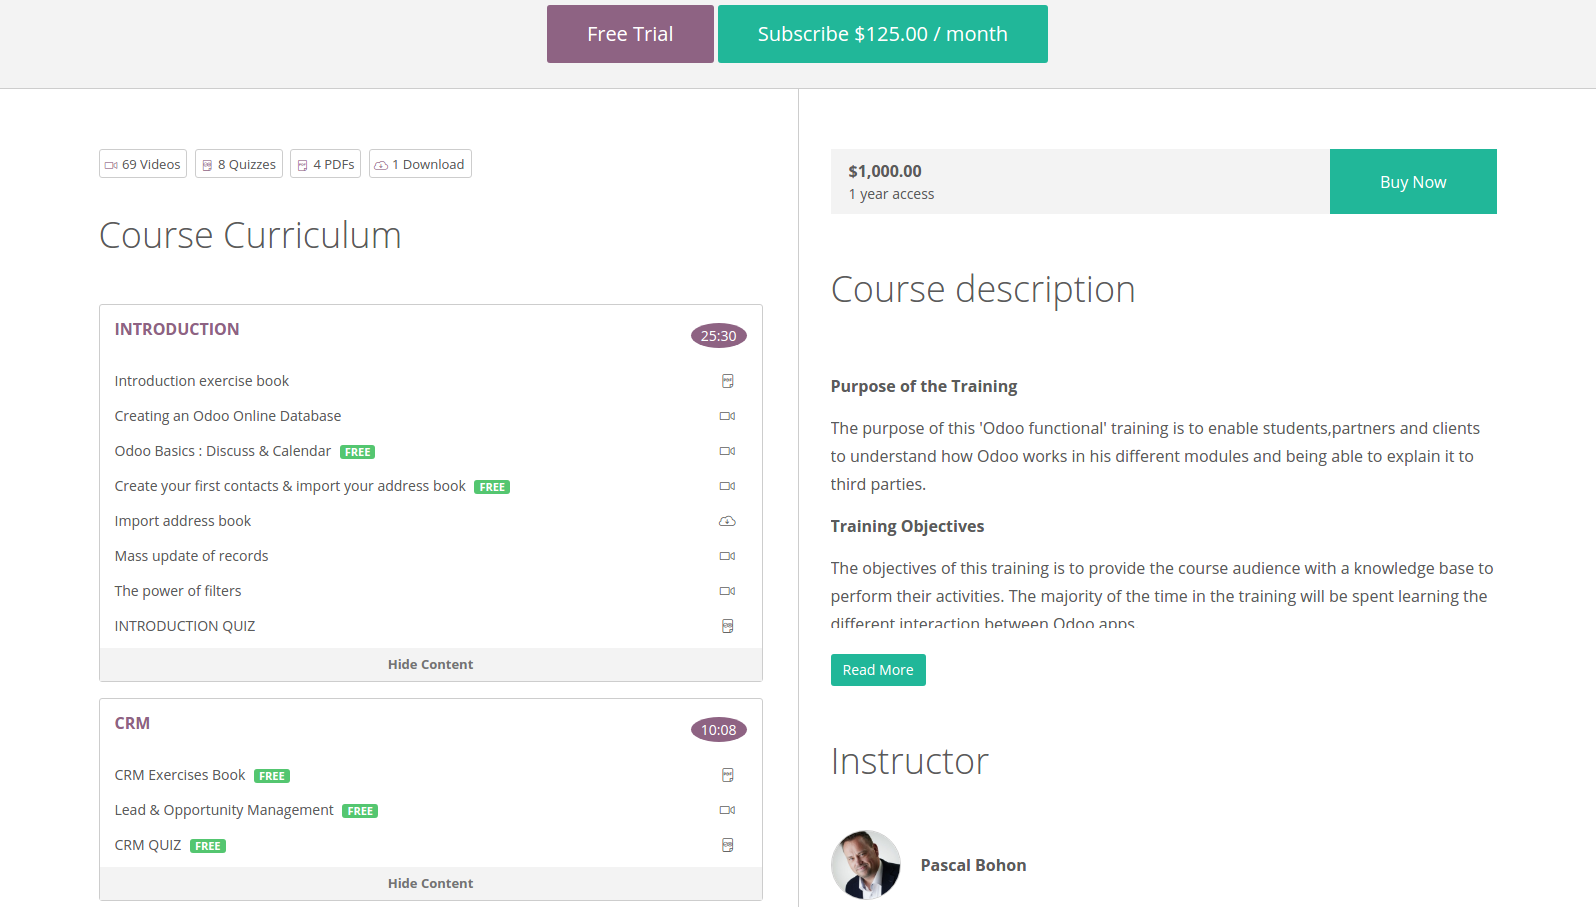
\includegraphics[width=12cm]{../pics/odoosatraining}
		\caption{\href{https://odoo.thinkific.com/courses/odoo-functional}{Free trial (\cite{odoosatraining})}}
	\end{figure}
}

\frame{
	\frametitle{Odoo Training}
	\framesubtitle{ERP Courses on \href{http://edx.org}{edX}}
	\begin{figure}	
		\centering
		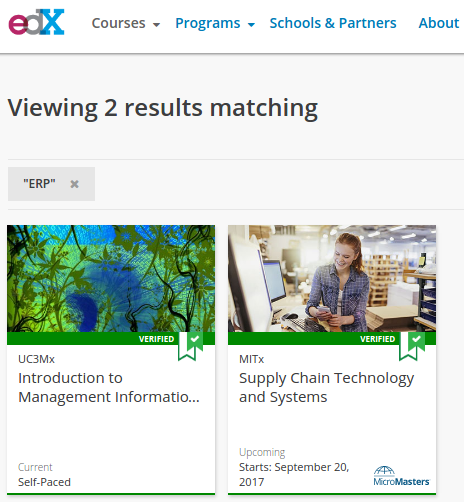
\includegraphics[height=6cm]{../pics/edx-ERP-courses}
		\caption{Top courses available at \href{http://edx.org}{edX}}
	\end{figure}
}

% ~ ~ ~ References
% ======================================================================================================
%                                     References
% ======================================================================================================
\section{References}
\frame[allowframebreaks]{
	\frametitle{Odoo: the course ERP}
	\framesubtitle{References}
	% keyword refers to bib file: references-KEYWORD.bib, and to the Tex file: section-KEYWORD.tex
	\printbibliography[keyword=odoo-course-erp]
}




\end{document}

